\documentclass[conference]{IEEEtran}
\usepackage[english]{babel}
\usepackage{cite,setspace}
\usepackage[autostyle]{csquotes}
\usepackage{amsmath,amssymb,amsfonts}
\usepackage{algorithmic}
\usepackage{graphicx}
\graphicspath{{images/}}
\usepackage{textcomp}
\usepackage{xcolor}
\usepackage[outputdir=output]{minted}
%\usemintedstyle{autumn} % friendly, colorful
%\newminted{c}{mathescape, linenos, numbersep=5pt, gobble=0, frame=lines, framesep=2mm}
%\definecolor{background}{gray}{0.90}
%\newminted{bash}{bgcolor=background}
%\newminted{console}{bgcolor=background}
%\usemintedstyle[console]{bw}
\def\BibTeX{{\rm B\kern-.05em{\sc i\kern-.025em b}\kern-.08em
    T\kern-.1667em\lower.7ex\hbox{E}\kern-.125emX}}
\begin{document}

\title{A Study of Scene Semantics: Project 1}

\author{\IEEEauthorblockN{Mark Wesley Harris}
\IEEEauthorblockA{\textit{CS5800 Computer Graphics, Fall 2019} \\
\textit{University of Colorado Colorado Springs}\\
Colorado Springs, United States \\
wharris2@uccs.edu}}

\maketitle

\section{Introduction}
\label{sec:introduction}
Quality source material is key for a successful research project.
The proposed work of defining semantics for 3D scenes is no exception to this rule;
a powerful computer and complex animation source file are both required
for good research on this topic.
Described here are the steps taken for setting up the project
source materials and environment, as well as discussion on future steps
for how to use these sources for researching scene semantics.

\section{Work Accomplished}
\label{sec:work}

\subsection{Computer Build}
\label{subsec:build}
A new computer was built at the start of the semester, in order to better prepare for the necessary machine learning
research and graphical image processing. One RTX 2060 GPU was purchased,
since the 2060 model is the cheapest GPU that also has Tensor cores
(which are useful specifically for training machine learning models).
The processor chosen was the AMD RYZEN 3600.
All the components were assembled,
and the result was a well-equipped computer running Windows 10 Pro.

Autodesk Maya 2019 student edition
and RenderMan 22 were
installed as the animation and rendering softwares for the project.
Since RenderMan is maintained by Pixar Animation Studios and not a software solution company
(like Maya),
tutorials and walkthroughs were somewhat hard to find. One tutorial which helped get the foundation
of the work started was \cite{renderman}.

\subsection{Modeling}
The ``table'' that was modeled is shown in Figure \ref{fig:environment}.
To model one ring of the table, a primitive cylinder was flattened.
Its rim was extruded, and the inside raised slightly to create a more interesting object.
This new disk primitive was copied twice in order to form the two inside-portions of the table.
Sphere primitives were used to create the half-dome on top of the outer-table, and the centerpiece
that rests inside. 12 cylinders were used for the legs, and cylinders were also used
for the hinges that join the tables together.

\begin{figure}[htbp]
\centerline{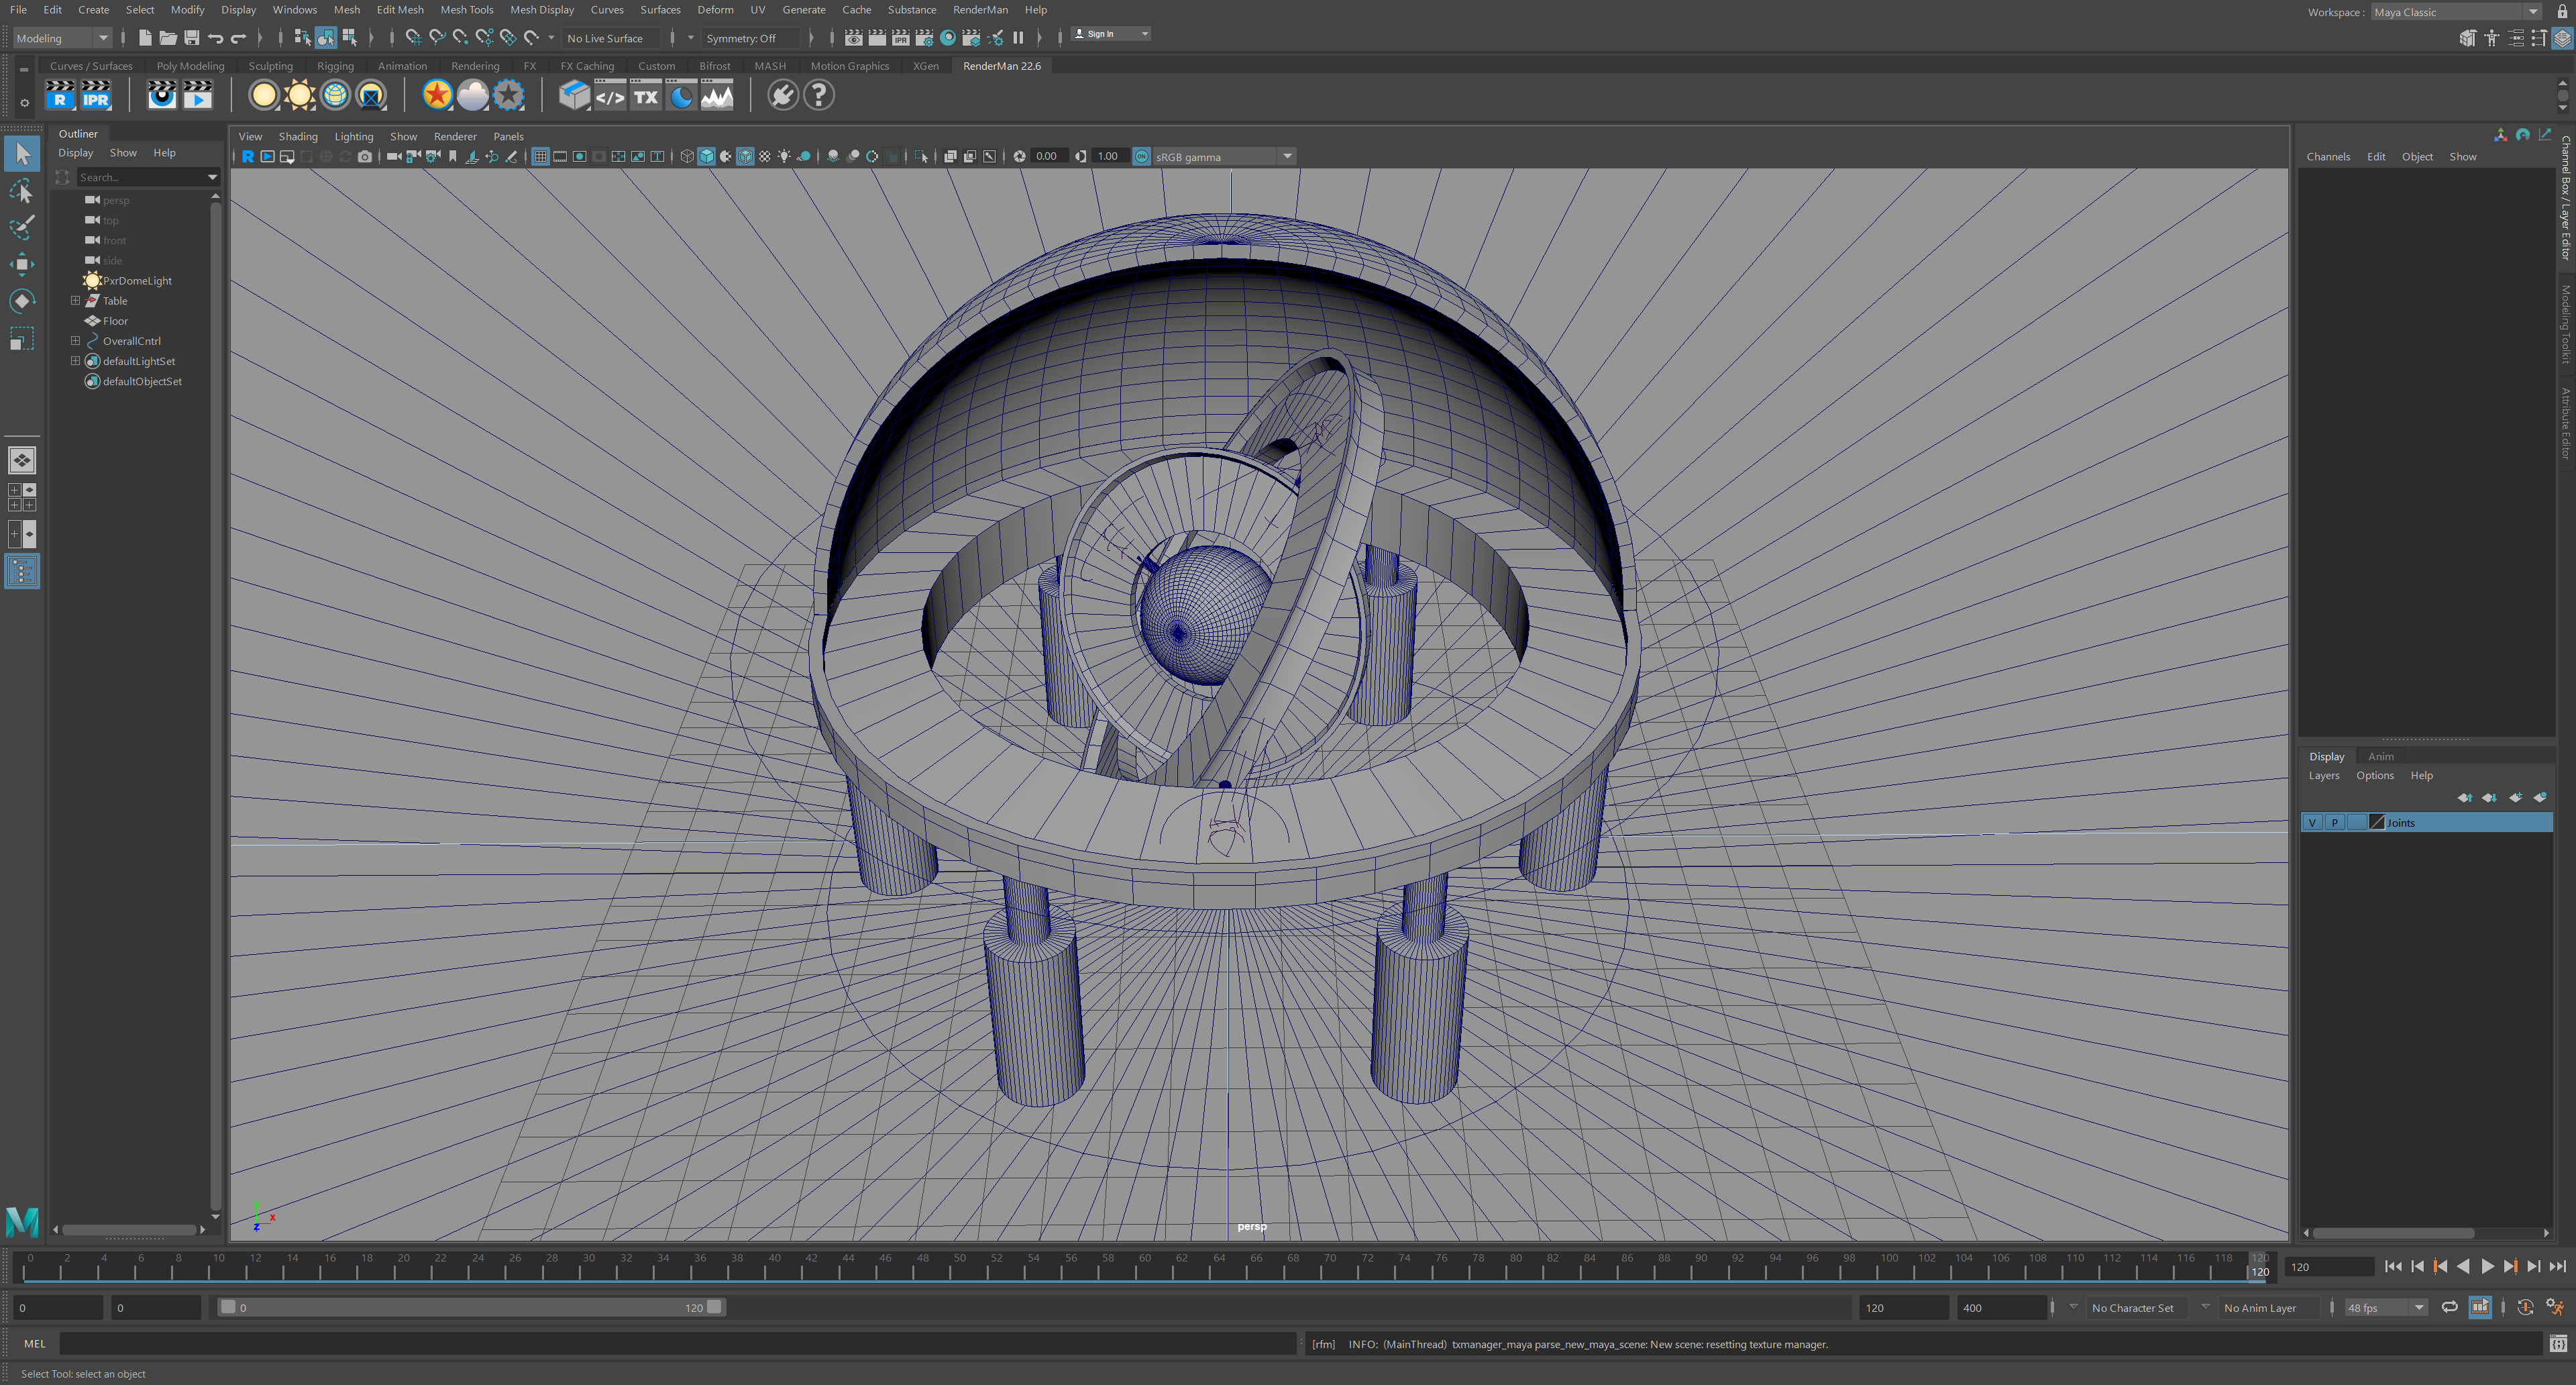
\includegraphics[width=8.5cm]{project1.png}}
\caption{``Table'' source in Autodesk Maya.}
\label{fig:environment}
\end{figure}

Many materials were experimented with. As discussed in \cite{renderman},
RenderMan comes with a shelf of unique material presets that may be further customized as desired.
Instead of choosing one to customize for each part of the table,
many different materials were used in order to obtain the most dynamic render possible.
All components besides the floor and center sphere were transparent, with varying indices of refraction.
The result was a complex scene with a considerably long render-time.
Using the computer discussed in Section \ref{subsec:build},
rendering a single HD (1920 x 1080) frame took around 15 minutes to complete.

\subsection{Animation}
In order to animate the scene, joints were placed at each hinge and parented to the object groups they operate.
Control objects were then created and constrained for each joint group,
so that the joints themselves were left unaltered throughout animation \cite{rigging}.
In total, 5 control objects were used to animate the joints in the scene.
Keyframes were added over the course of 120 frames, and made to loop smoothly.

Since rendering a frame takes about 15 minutes,
rendering the entire 120 frame sequence took approximately 30 hours to complete.
Each frame was then placed into a slideshow and exported in movie format at 30 frames per second.
This created an animation around 5 seconds long,
but with plenty of movement and dynamic material interaction.
One of the final rendered frames of the animated sequence is shown in Figure \ref{fig:table}.
The animation itself is posted on YouTube \cite{animation}.

\begin{figure*}[htbp]
\centerline{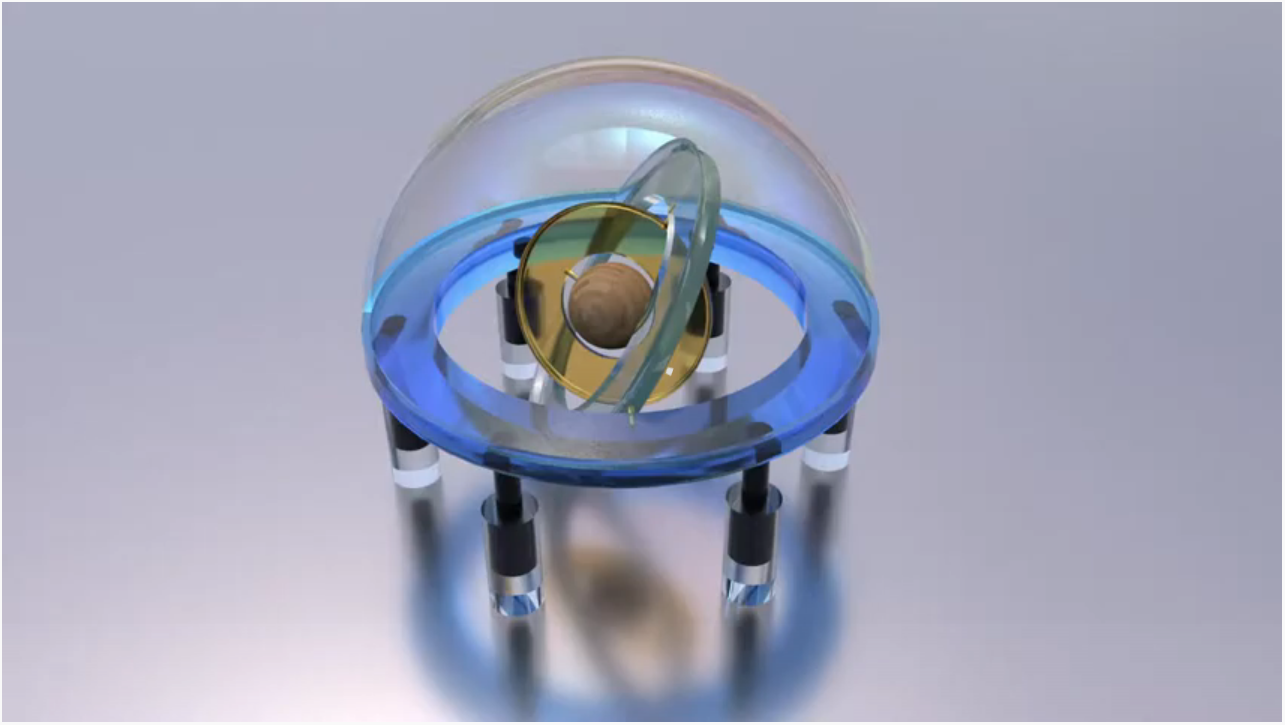
\includegraphics[width=18cm]{table.png}}
\caption{``Table'' animated with Autodesk Maya and rendered with RenderMan \cite{animation}.}
\label{fig:table}
\end{figure*}

\section{Future Work}
\label{sec:future}
There are several more steps to complete throughout the semester.
Now that the environment and scene have been set up for the project,
the RenderMan research can be started.
General steps are listed below in chronological order.
\begin{enumerate}
\item Research how to interact with the RenderMan Interface.
\item Collect as much data as possible from shaders through this interface or by other means.
\item Optimize the collection so that generalizations from the scene can be made at each pixel.
\item Research export mechanisms for exporting the information from the scene.
\end{enumerate}
It is unknown how long any of the listed items will take.
There is an expectation for either less or extra work to be completed,
given the difficulties encountered while exploring solutions.
These will be noted in future reports.

\section{Conclusion}
\label{sec:conclusion}
The foundations of the proposed project have been completed.
A qualifying computer was built, and a basic environment installed.
Then a dynamic scene was animated in Autodesk Maya and exported
using RenderMan. Research into collecting semantics from the scene using
the RenderMan Interface and RenderMan Shading Language (RSL)
will be the focus of the project from now on.

\bibliography{project}
\bibliographystyle{IEEEtran}

%==========================================================
\end{document}
%==========================================================
